\documentclass[journal,12pt,twocolumn]{IEEEtran}
\usepackage{hyperref}
\usepackage{graphicx}
\usepackage{enumitem}
\usepackage{amsmath}
\usepackage{amssymb}
\title{Assignment: Random numbers}
\author{JARPULA BHANU PRASAD - AI21BTECH11015}
\date{June 2022}
\begin{document}
\maketitle
\newcommand{\solution}{\noindent \textbf{Solution: }}

\section{\underline{Uniform Random Numbers}}
Let $U$ be a uniform random varaible between 0 and 1.
\begin{itemize}
    \item \textbf{1.1} Generate $10^6$ samples of $U$ using a C program and save into a file called uni.dat .\\
    \solution Download the following files and execute the C program \\
    The C code - \href{https://github.com/jarpula-Bhanu/Random-numbers/blob/main/codes/exrand.c}{exrand.c} \\
    The Header - \href{https://github.com/jarpula-Bhanu/Random-numbers/blob/main/codes/coeffs.h}{coeffs.h} \\ 
    \\Compile and execute the above C program using command
    \begin{itemize}
        \item gcc exrand.c -lm -o exrand.out
        \item ./exrand.out \\
    \end{itemize}
    
    \item \textbf{1.2} Load the uni.dat file into python and pot the empirical CDF of $U$ using the samples in uni.dat . The CDF is defined as 
    \begin{align}
        F_U(x) = Pr(U \le x)
    \end{align}
    \solution The following code plots Fig. \ref{fig:uni_cdf}
    \\
    Python code - \href{https://github.com/jarpula-Bhanu/Random-numbers/blob/main/codes/cdf_plot.py}{cdf\_plot.py} \\
    The above code is executed using command
    \begin{itemize}
        \item python3 cdf\_plot.py
    \end{itemize}
    \begin{figure}[h]
        \centering
        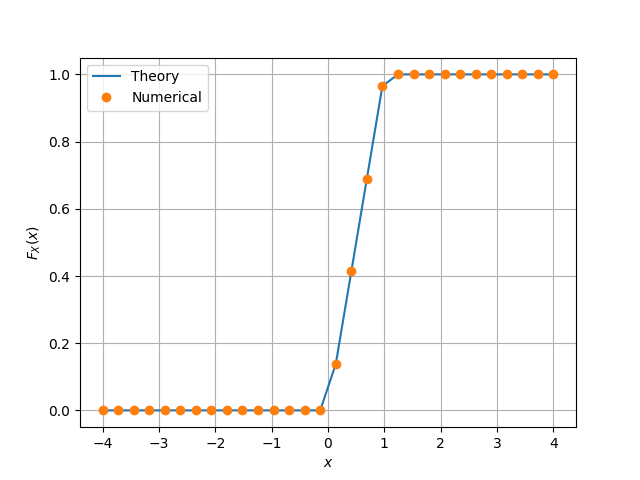
\includegraphics[width=\columnwidth]{uni_cdf.png}
        \caption{The CDF of $U$}
        \label{fig:uni_cdf}
    \end{figure}

    \item \textbf{1.3} Find the theoritical expression for $F_U(x)$. \\
    \solution Since $U$ is a uniformly distributed in [0,1]  \\
    We have three cases:
	\begin{itemize}
	\item $x < 0$: $P_X(x) = 0$, and hence $F_U(x) = 0$.
	\item $0 \leq x < 1$: Here,
	\begin{align}
        F_U(x) = \int_{0}^{x}du = x
	\end{align}
	\item $x \geq 1$: Put $x = 1$ in above eqn we get $F_U(x) = 1$.
	\end{itemize}
Therefore,
    \begin{align}
		F_U(x) = 
		\begin{cases}
			0 & x < 0 \\
			x & 0 \leq x < 1 \\
			1 & x \geq 1
		\end{cases}
    \end{align}
This can be verified from Fig. \ref{fig:uni_cdf} \\
    
    \item \textbf{1.4} The mean of $U$ is defined as 
    \begin{align}
        E[U] = \frac{1}{N} \sum_{i=1}^N U_i
    \end{align}
    and its varaience as 
    \begin{align}
        var[U] = E[U - E[U]]^2
    \end{align}
    Write a C program to find the mean and varaience of $U$ \\
    
    \solution Download and run the following C code.\\
    Mean and varaience - \href{https://github.com/jarpula-Bhanu/Random-numbers/blob/main/codes/mean-var1-4.c}{mean-var1-4.c}\\
    The Header - \href{https://github.com/jarpula-Bhanu/Random-numbers/blob/main/codes/coeffs.h}{coeffs.h} \\
    \\Compile and execute the above C program using command
    \begin{itemize}
        \item gcc mean-var1-4.c -lm -o mean-var1-4.out
        \item ./mean-var1-4.out \\
    \end{itemize}

    \item \textbf{1.5} Verify your result theotically given that 
    \begin{align}
        E[U^k] = \int_{-\infty}^{\infty} x^k dF_U(x) 
    \end{align}
    \solution Verifying result theoritically\\
    Given that
    \begin{align}
        E[U^k] &= \int_{-\infty}^{\infty} x^k dF_U(x)
    \end{align}
    Mean is given by
    \begin{align}
        E[U] &= \int_{-\infty}^{\infty} x dF_U(x) \\
        &= \int_{-\infty}^{\infty} x dx \\
        &= \bigg[\frac{x^2}{2}\bigg]_0^1 \\
        &= \frac{1}{2}
    \end{align}
    Varaience is given by
    \begin{align}
        E[U-E[U]]^2 &= E[U^2] - E[U]^2 \\
        E[U]^2 &= \int_{-\infty}^{\infty} x^2 dF_U(x)\\
        &= \int_{-\infty}^{\infty} x^2 dx \\
        &= \bigg[\frac{x^3}{3}\bigg]_0^1 \\
        &= \frac{1}{3} \\
        E[U-E[U]]^2 &= \frac{1}{3} - (\frac{1}{2})^2 \\
        &= \frac{1}{3} - \frac{1}{4} \\
        &= \frac{1}{12}
    \end{align}
\end{itemize}

\section{\underline{Central Limit Theorem}}

\begin{itemize}
    \item \textbf{2.1} Generate $10^6$ samples of the random varaible 
    \begin{align}
        X = \sum_{i=1}^{12} U_i - 6
    \end{align}
    Using a C program, where $U_i$ = 1,2,.........12 are a set of independent uniform random variables between 0 and 1 and save in a file called gau.dat \\
    \solution Download the following files and execute the C program \\
    The C code - \href{https://github.com/jarpula-Bhanu/Random-numbers/blob/main/codes/exrand.c}{exrand.c} \\
    The Header - \href{https://github.com/jarpula-Bhanu/Random-numbers/blob/main/codes/coeffs.h}{coeffs.h} \\ 
    \\Compile and execute the above C program using command
    \begin{itemize}
        \item gcc exrand.c -lm -o exrand.out
        \item ./exrand.out \\
    \end{itemize} 

    \item \textbf{2.2} Load gau.dat in python and plot the empirical CDF of $X$ using the sample in gau.dat. What properties does a CDF have? \\
    \solution The CDF of $X$ is plotted in Fig. \ref{fig:gauss_cdf}
    \begin{figure}[h]
        \centering
        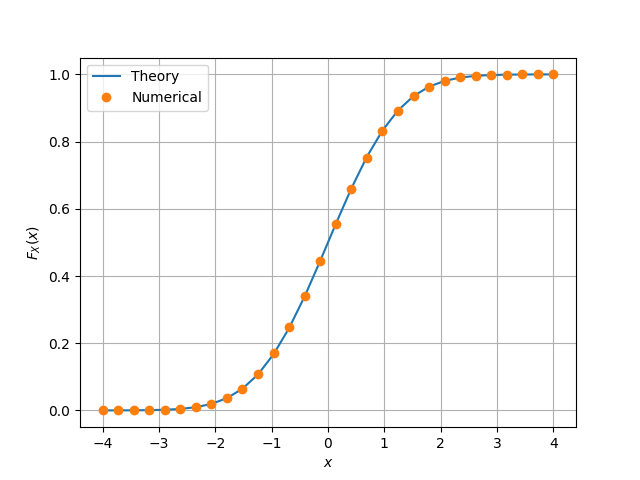
\includegraphics[width=\columnwidth]{gauss_cdf.png}
        \caption{The CDF of $X$}
        \label{fig:gauss_cdf}
    \end{figure}
    \textbf{properties of cdf}
    \begin{itemize}
        \item $F_X(x)$ is a nondecreasing function of x for -$\infty < x < \infty$. 
        \item The CDF, $F_X(x)$ ranges from 0 to 1. This makes sense since $F_X(x)$ is a probability.
        \item If the maximum value of $X$ is b,\\ then $F_X(b)$ = 1 \\
    \end{itemize} 
    
    \item \textbf{2.3} Load gau.dat in python and plot the empirical PDF of $X$ using the samples in gau.dat. The PDF of $X$ is defined as 
    \begin{align}
        P_X(x) = \frac{d}{dx} F_X(x)
    \end{align}
    What properties does the PDF have? \\
    \solution The PDF of $X$ is plotted in Fig. \ref{fig:gauss_pdf}
    using the code below \\
    Python code - \href{https://github.com/jarpula-Bhanu/Random-numbers/blob/main/codes/pdf_plot.py}{pdf\_plot.py}\\
    The above code is executed using command
    \begin{itemize}
        \item python3 pdf\_plot.py \\
    \end{itemize}
    \begin{figure}[h]
        \centering
        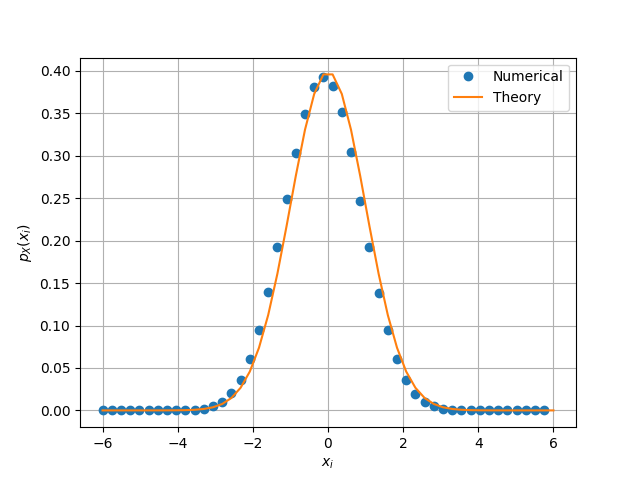
\includegraphics[width=\columnwidth]{gauss_pdf.png}
        \caption{The PDF of $X$}
        \label{fig:gauss_pdf}
    \end{figure}
    
    \textbf{properties of pdf}
    \begin{itemize}
        \item PDF is symmetric about $X$ = 0 
        \item Graph is bell shaped
        \item Mean of graph is situated at the apex point of the bell.\\
    \end{itemize}
    
    \item \textbf{2.4} Find the mean and varaience of $X$ by writing a C program.\\
     
    \solution Download and run the following C code.\\
    Mean and varaience - \href{https://github.com/jarpula-Bhanu/Random-numbers/blob/main/codes/mean-var2-4.c}{mean-var2-4.c}\\
    The Header - \href{https://github.com/jarpula-Bhanu/Random-numbers/blob/main/codes/coeffs.h}{coeffs.h} \\
    \\Compile and execute the above C program using command
    \begin{itemize}
        \item gcc mean-var2-4.c -lm -o mean-var2-4.out
        \item ./mean-var2-4.out \\
    \end{itemize} 
    
    \item \textbf{2.5} Given that 
    \begin{align}
        P_X(x) = \frac{1}{\sqrt{2\pi}}e^{(-\frac{x^2}{2})}, -\infty < x < \infty
    \end{align}
    repeat the above exercise theoritically.\\
    \solution Verifying theoritically
    \begin{align}
        F_X(x) &= \int_{-\infty}^{x}\frac{1}{\sqrt{2\pi}}e^{-\frac{x^2}{2}}dx \\
        &= \frac{1}{2} erf\bigg(\frac{x}{\sqrt{2}}\bigg)\\
        E[X]&= \frac{1}{\sqrt{2\pi}} \int_{-\infty}^{\infty}xe^{-\frac{x^2}{2}}dx 
    \end{align}
    Taking $\frac{x^2}{2} = t \rightarrow xdx = dt$
    \begin{align}
        E[X]&= \frac{1}{\sqrt{2\pi}} \int_{-\infty}^{\infty}e^{-t} dt = 0 \\
        E[X^2]&= \frac{1}{\sqrt{2\pi}} \int_{-\infty}^{\infty}x^2e^{-\frac{x^2}{2}}dx \\
        &= \frac{1}{\sqrt{2\pi}} \int_{-\infty}^{\infty}x(xe^{-\frac{x^2}{2}})dx \\
        &= \frac{1}{\sqrt{2\pi}} \bigg[-xe^{\frac{x^2}{2}}+\int_{-\infty}^{\infty}e^{-\frac{x^2}{2}} dx \bigg] \\
        &= 1 \\
        \textbf{variance} &= E[X^2] - E[X]^2 = 1
    \end{align}
\end{itemize}

\section{\underline{From uniform to other}}
\begin{itemize}
    \item \textbf{3.1} Generate samples of 
    \begin{align}
        V = -2 ln(1-U)
    \end{align}
    and plot its CDF. \\
    \solution Download the following files and execute the C program \\
    The C code - \href{https://github.com/jarpula-Bhanu/Random-numbers/blob/main/codes/exrand.c}{exrand.c} \\
    The Header - \href{https://github.com/jarpula-Bhanu/Random-numbers/blob/main/codes/coeffs.h}{coeffs.h} \\ 
    \\Compile and execute the above C program using command
    \begin{itemize}
        \item gcc exrand.c -lm -o exrand.out
        \item ./exrand.out \\
    \end{itemize} 
    The above C program will save the values of V in log.dat \\ 
    \\The CDF of $X$ is plotted in Fig. \ref{fig:V_cdf}
    using the code \\
    Python code - \href{https://github.com/jarpula-Bhanu/Random-numbers/blob/main/codes/cdf_plot3-1.py}{cdf\_plot3-1.py} \\
    The above code is executed using command
    \begin{itemize}
        \item python3 cdf\_plot3-1.py\\
    \end{itemize}

    \begin{figure}[h]
        \centering
        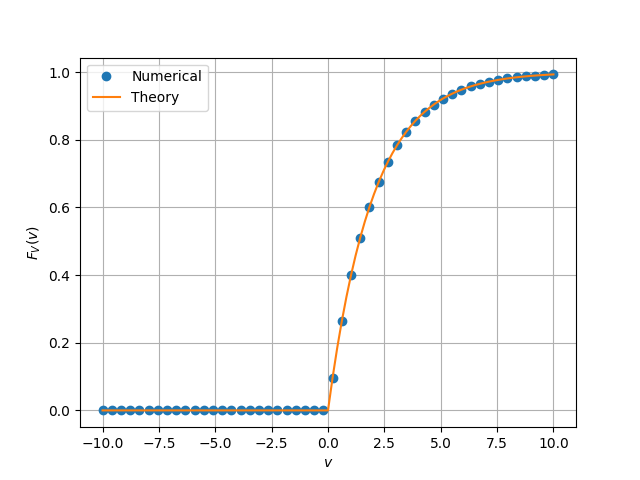
\includegraphics[width=\columnwidth]{V_cdf.png}
        \caption{The CDF of $V$}
        \label{fig:V_cdf}
    \end{figure}

    \item \textbf{3.2} Find a theoritical expression for $F_V(x)$. \\
    \solution 
    \begin{align}
        F_V(x) &= Pr(V \le x)\\
        &= Pr(-2 ln(1-U) \le x) \\
        &= Pr(U \le 1-e^{-\frac{x^2}{2}}) \\
        Pr(U<x) &= \int_0^x dx = x \\
        \therefore Pr(U \le 1-e^{-\frac{x^2}{2}}) &= 1-e^{-\frac{x^2}{2}} \\
        \rightarrow F_V(x) &=1-e^{-\frac{x^2}{2}}
    \end{align}
\end{itemize}

\end{document}